\documentclass[../analysisII_notes.tex]{subfiles}
\begin{document}
\section{Aula 05 - 17 de Março, 2025}
\subsection{Motivações}
\begin{itemize}
	\item Propriedades da Integral;
	\item Algumas Funções para testar.
\end{itemize}
\subsection{Propriedades da Integral}
Vamos recapitular nossos interesses até aqui: estamos estudando o problema de determinar a ``área sob o gráfico'' de uma função limitada, definida num intervalo fechado e limitado, Para isso,
fomos atrás dos conceitos de soma superior e inferior desta função, mas associadas a uma partição do intervalo - pontos escolhidos manualmente para serem levados como base. A partir da partição e da soma, coletamos, em conjuntos,
os valores mais altos e mais baixos possíveis destas somas para cada partição, com uma delas pecando pela falta da área (cobriu menos área que a função), e outra pelo excesso (cobriu mais área que a função). Pegando os extremos destes conjuntos, foi natural
introduzir as integrais como
\begin{itemize}
	\item[i)] A melhor aproximação da área desejada por falta:
	      \[
		      \underline{\intup_{a}^{b}}f(x)dx = \sup_{}\sigma (f);
	      \]
	\item[ii)] A melhor aproximação por excesso:
	      \[
		      \overline{\intup_{a}^{b}}f(x)dx=\inf_{}\Sigma (f).
	      \]
\end{itemize}
A ideia do porquê disso fazer sentido é que, pegando os extremos destes intervalos, estamos pegando partições cada vez mais refinadas e somas cada vez mais próximas do valor real da área - aqui entra o teorema da aula 3. A partir disso,
definimos a integral como o valor quando a melhor aproximação que peca pelo excesso e a melhor que peca pela falta, coincidem! f é integrável em \([a, b]\), e escrevemos \(f\in \mathcal{R}([a, b])\), quando
\[
	\overline{\intup_{a}^{b}}f = \underline{\intup_{a}^{b}} f = \int_{a}^{b},
\]
e este valor comum é chamado integral de f em \([a, b]\). Após chegarmos a esta definição, vimos alguns exemplos para solidificar os conceitos.

Nosso próximo passo, então, acaba sendo relacionado a identificar as funções integráveis, junto às que não são, até finalmente conseguirmos caracterizá-las por completa\footnote{Spoiler: será com base nos seus pontos de continuidade, mas a função não precisa ser contínua! Lembre-se dos conceitos de descontinuidades de primeira e segunda ordem para entender isso :).}

Para facilitar esta árdua tarefa, veremos como fazer para operacionalizar a integral, ou seja, como o valor da integral se comporta quando submetemos as funções às somas e produtos por escalares\footnote{Como apontou o Édinho, não se sabe de uma relação quanto ao produto e divisão de funções, especialmente para a integral definitiva. Uma forma de ver por que olhamos para a soma e produto escalar é que a integral definitiva consiste em um \textit{funcional linear} do espaço de funções à reta real!}. Comecemos demonstrando uma desigualdade muito bem ilustrada nos desenhos:
\begin{prop*}
	Se \(f:[a, b]\rightarrow \mathbb{R}\) é limitada, então
	\[
		\underline{\intup_{a}^{b}}f \leq \overline{\intup_{a}^{b}}f.
	\]
\end{prop*}
\begin{proof*}
	Com efeito, sabemos, da aula passada, que
	\[
		L(f; \mathcal{P}) \leq U(f, \mathcal{Q})
	\]
	para todas as partições \(\mathcal{P},\: \mathcal{Q}\) de um intervalo \([a, b]\). Sendo assim, fixada uma partição \(\mathcal{P}\), a soma inferior \(L(f; \mathcal{P})\) é cota inferior de \(\Sigma (f)\). Destarte,
	\[
		L(f; \mathcal{P})\leq \overline{\intup_{a}^{b}}f = \inf_{}\Sigma (f),
	\]
	já que a integral superior é a maior das cotas inferiores.

	Por outro lado, isto também siginfica que \(\sigma(f)\) é cota superior de \(\sigma (f)\), pois \(\mathcal{P}\) foi uma partição selecionada abitrariamente. Em particular, ela é uma cota superor maior do que a menor cota superior de \(\sigma (f)\) (afinal, a menor é a menor), que é a integral infeiror de f dentro do intervalo
	Portanto,
	\[
		\underline{\intup_{a}^{b}}f \leq \overline{\intup_{a}^{b}}f.\quad \text{\qedsymbol}
	\]
\end{proof*}
Com este resultado, inauguramos as operações das integrais! A primeira delas que estabeleceremos é que, se \(f:[a, b]\rightarrow \mathbb{R}\) é limitada e c é um valor entre a e b, então
\[
	\underline{\intup_{a}^{b}}f = \underline{\intup_{a}^{c}}f + \underline{\intup_{c}^{b}}f \quad\&\quad \overline{\intup_{a}^{b}}f = \overline{\intup_{a}^{c}}f + \overline{\intup_{c}^{b}}f.
\]
O que isto quer dizer é que, ao calcular a integral, a pessoa pode selecionar algum ponto no intervalo e usar ele de ``ponto de corte'': as integrais à direita referem-se às integrais das funções restritas aos intervalos \([a, c]\) e \([c, b]\):
\begin{align*}
	 & f|_{[a, c]}:[a, c]\rightarrow \mathbb{R}  \\
	 & f|_{[c, b]}:[c, b]\rightarrow \mathbb{R}.
\end{align*}
\begin{figure}[H]
	\begin{center}
		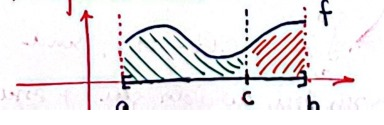
\includegraphics[height=0.5\textheight, width=0.5\textwidth, keepaspectratio]{./Images/cut_interval_05.png}
	\end{center}
	\caption{ao calcular a integral, podemos escolher um ponto de corte e separar a função em duas (ou mais, se reptirmos isto cada vez mais) metades.}
	\label{cutint05}
\end{figure}

Quanto à prova disto, precisaremos de dois resultados: um sobre supremos e ínfimos; outro, sobre integrais superior e inferior.
\begin{lemma*}
	Sejam A' e B' respectivos subconjuntos de conjuntos não-vazios A, limitdado superiormente, e B, limitado inferiormente, ambos consistindo de números reais. Então,
	\begin{itemize}
		\item[i)] Se, para todo elemento de A, existir um elemento em A' maior ou igual que o de A, então os supremos coincidem; em termos simbólicos:
		      \[
			      \forall a\in A,\: \exists a'\in A': a\leq a' \Rightarrow \sup_{}A = \sup_{}A'.
		      \]
		\item[ii)] Analogamente, se para todo elemento de B, existir um elemento em B' menor ou igual ao de B, então os ínfimos coincidem:
		      \[
			      \forall b\in B,\: \exists b'\in B': b\geq b' \Rightarrow \inf_{}B = \inf_{}B'.
		      \]
	\end{itemize}
\end{lemma*}
\begin{proof*}
	Provaremos o item (i), deixando o (ii) como exercício

	Em primeiro lugar, pelas propriedades normais de supremo,
	\[
		\sup_{}A' \leq \sup_{}A,
	\]
	pois, o supremo de A é cota superior de A', então deve ser maior do que a menor cota superior de A'.

	A fim de contradição, suponha que \(\sup_{}A'=\sup_{}A\) não ocorre, restando apenas a desigualdade estrita; logo, \(\sup_{}A'\) não pode ser cota superior de A, já que o supremo de A já é a menor delas. Consequentemente, existe um elemento a em A com
	\[
		\sup_{}A' < a.
	\]
	Porém, por hipótese, existe um elemento a' de A' que corresponde ao a e que satisfaz \(a\leq a'\); em particular,
	\[
		\sup_{}A' < a \leq a',
	\]
	uma contradição! Portanto, a igualdade deverá prevalecer. \qedsymbol
\end{proof*}
\begin{exr}
	Prove o item (ii) do lema acima.
\end{exr}

O grande ganho deste primeiro lema é que, ao encontrar conjuntos satisfazendo as hipóteses postuladas, podemos nos restringir a eles para calcular o supremo e o ínfimo. Por exemplo,
\begin{example}
	Considere os conjuntos
	\[
		B=\biggl\{\frac{1}{n}:\: n\in \mathbb{N}\biggr\} \quad\&\quad B'=\biggl\{\frac{1}{2n}:\: n\in \mathbb{N}\biggr\}.
	\]
	Temos \(B'\subseteq B\), B limitado inferiormente e, se a for um elemento de B com forma \(1/n\), basta tomar o elemento a' de B´ dado por \(1/2n\) que cumprimos a hipótese do enunciado do lema. Portanto,
	\[
		\inf_{}B' = \inf_{}B = 0.
	\]
\end{example}
\begin{theorem*}
	Se \(\mathcal{P}_{0}\) é uma partição qualquer do intervalo \([a, b]\) e \(f:[a, b]\rightarrow \mathbb{R}\) é uma função limitada, então
	\begin{align*}
		 & \text{(I) } \underline{\intup_{a}^{b}}f = \sup_{\mathcal{P}\supseteq \mathcal{P}_{0}}L(f; \mathcal{P})  \\
		 & \text{(II) } \overline{\intup_{a}^{b}}f = \inf_{\mathcal{P}\supseteq \mathcal{P}_{0}}U(f; \mathcal{P}).
	\end{align*}
	Noutras palavras, para calcular as integrais acima, podemos nos restringir às partições que refinam alguma outra.
\end{theorem*}
\begin{proof*}
	Vamos fazer Penas a prova de (II), pois a (I) segue de forma análoga. Com efeito, denote por
	\[
		B'\coloneqq \{U(f; \mathcal{Q}):\: \mathcal{Q}\supseteq \mathcal{P}_{0}\} \quad\&\quad B\coloneqq \Sigma (f),
	\]
	tal que \(B'\) é subconjunto de \(B\) (nosso objetivo é aplicar o lema, e esta notação deixará mais claro a forma que ele aparece). Agora, se \(\mathcal{P}\) for uma partição qualquer de \([a, b]\), então como
	\[
		\mathcal{P}\cup \mathcal{P}_{0}\supseteq \mathcal{P}_{0},
	\]
	segue que
	\[
		U(f; \mathcal{P}\cup \mathcal{P}_{0})\in \{U(f; \mathcal{Q}): \mathcal{Q}\supseteq \mathcal{P}_{0}\},
	\]
	com
	\[
		U(f; \mathcal{P}\cup \mathcal{P}_{0}) \leq U(f; \mathcal{P}).
	\]
	Portanto, pelo item (ii) do Lema,
	\[
		\inf_{\mathcal{Q}\supseteq \mathcal{P}_{0}}U(f; \mathcal{Q}) = \inf_{}\Sigma (f)=\overline{\intup_{a}^{b}}f.\quad \text{\qedsymbol}
	\]
\end{proof*}
\begin{def*}
	Se A, B são subconjuntos da reta real, seu \textbf{conjunto-soma} é definido como
	\[
		A+B\coloneqq \{a+b:\:a\in A\:b\in B\}.\quad \square
	\]
\end{def*}
\begin{example}
	Se \(A=\{1, 2\}\) e \(B=\{1, 3\}\), então o conjunto-soma de A com B é dado por
	\[
		A+B=\{1+1,1+3,2+1,2+3\}=\{2,4,3,5\}.
	\]
\end{example}
\begin{lemma*}
	Com a notação acima,
	\begin{itemize}
		\item[1)] Se A e B são limitados superiormente, então assim o é A+B e, além disso,
		      \[
			      \sup_{}(A+B)=\sup_{}A + \sup_{}B.
		      \]
		\item[2)] Se A e B são limitados inferiormente, então assim o é A+B e, além disso,
		      \[
			      \inf_{}(A+B)=\inf_{}A + \inf_{}B.
		      \]
	\end{itemize}
\end{lemma*}
\begin{proof*}
	Tome x como um elemento de A+B; então, existem elementos a de A e b de B tais que
	\[
		x=a+b.
	\]
	Sendo assim, como a e b são menores que os supremos de seus respectivos conjuntos,
	\[
		x = a+b \leq \sup_{}A + \sup_{}B.
	\]
	Isto basta para provar que A+B é limitado superiormente e, de quebra, que \(\sup_{}A+\sup_{}B\) é cota superior dele.

	Em seguida, para ver que é a menor cota superior, tome um \(\varepsilon \) positivo qualquer; existirão elementos a de A e b de B com
	\[
		\sup_{}A - \frac{\varepsilon }{2}<a \quad\&\quad \sup_{}B-\frac{\varepsilon }{2}<b.
	\]
	Logo, \(x\) definido como a soma de a com b pertence ao conjunto A+B e, além disso, cumpre
	\[
		(\sup_{}A+\sup_{}B)-\varepsilon <a+b = x,
	\]
	provando que
	\[
		\sup_{}(A+B)=\sup_{}A+\sup_{}B.\quad \text{\qedsymbol}
	\]
\end{proof*}
\begin{exr}
	Prove o item (II) do lema acima.
\end{exr}
Uma consequência extremamente importante deste lema é a seguinte à notação a seguir: se X é um subconjunto qualquer da reta real e \(f:X\rightarrow \mathbb{R}\) é uma função limitada,
\begin{align*}
	 & \text{(i)} \: \inf_{}(f)=\inf_{}f(X)=\inf_{}\{f(x):\:x\in X\};  \\
	 & \text{(ii)} \: \sup_{}(f)=\sup_{}f(X)=\sup_{}\{f(x):\:x\in X\}.
\end{align*}
Desta forma,
\begin{crl*}
	Sejam \(f, g:X\rightarrow \mathbb{R}\) duas funções limitadas no domínio X da reta real. As seguintes desigualdades são verdadeiras:
	\begin{itemize}
		\item[1)] \(\sup_{}(f+g)\leq \sup_{}f+\sup_{}g\);
		\item[2)] \(\inf_{}(f+g)\geq \inf_{}f + \inf_{}g\).
	\end{itemize}
\end{crl*}
\begin{proof*}
	Quanto ao item (1), observe que, colocando
	\[
		A=f(X)\quad\&\quad B=g(X),
	\]
	então
	\[
		(f+g)(X)=\{f(x)+g(x):\:x\in X\}\subsetneq A+B.
	\]
	Destarte, através do item (I) do Lema anterior, vemos que
	\begin{align*}
		\sup_{}(f+g)=\sup_{}(f+g)(X) & \leq \sup_{}(A+B)      \\
		                             & =\sup_{}A+\sup_{}B     \\
		                             & \sup_{}(f)+\sup_{}(g).
	\end{align*}
	Portanto,
	\[
		\sup_{}(f+g)\leq \sup_{}f +\sup_{}g.\quad \text{\qedsymbol}
	\]
\end{proof*}
\begin{exr}
	Prove o item restante.
\end{exr}

\begin{example}
	É possível ocorrer a desigualdade estrita; basta, para isso, considerar as funções \(f(x)=x\) e \(g(x)=-x\), com \(x\) variando no intervalo \([-1, 1]\). Neste caso,
	\[
		f+g\equiv 0 \quad ((f+g)(x)=0\: \forall x\in [-1, 1]),
	\]
	tal que
	\[
		\sup_{}(f+g)= 0,
	\]
	enquanto que
	\[
		\sup_{}f = \sup_{}g = 1 \Rightarrow \sup_{}f + \sup_{}g = 2.
	\]
\end{example}

Finalmente, podemos provar o
\hypertarget{integral_additivity}{\begin{theorem*}[Aditividade da Integral]
		Sejam \(f:[a, b]\rightarrow \mathbb{R}\) uma função limitada e c um número entre os extremos do intervalo \([a, b]\). Valem:
		\begin{align*}
			 & \text{(i) } \underline{\intup_{a}^{b}}f = \underline{\intup_{a}^{c}}f + \underline{\intup_{c}^{b}}f \\
			 & \text{(ii) } \overline{\intup_{a}^{b}}f = \overline{\intup_{a}^{c}}f + \overline{\intup_{c}^{b}}f.
		\end{align*}
	\end{theorem*}}
\begin{proof*}
	Provaremos apenas o segundo. Todo o argumento se resume em observar que, para obter a integral superior de f, basta considerar as partições de \([a, b]\) que contêm o ponto c, isto é, aquelas que refinem a partição de três pontos
	\[
		\mathcal{P}_{0}: a < c < b,
	\]
	tal que,
	\[
		\overline{\intup_{a}^{b}}f = \inf_{\mathcal{P}\supseteq \mathcal{P}_{0}}U(f; \mathcal{P})
	\]
	e que, além disso, se \(\mathcal{Q}\) particiona o intervalo \([a, c]\) e \(\mathcal{R}\) o intervalo \([c, b]\), então \(\mathcal{P}=\mathcal{Q}\cup \mathcal{R}\) será uma partição do intervalo \([a, b]\) como um todo, contendo o ponto c.

	Reciprocamente, se \(\mathcal{P}\) particiona \([a, b]\) é uma partição contendo c, então podemos reescrevê-la como
	\[
		\mathcal{P}=(\mathcal{P}\cap [a, c])\cup (\mathcal{P}\cap [c, b]),
	\]
	sendo o primeiro termo em parênteses uma partição de \([a, c]\) e, o segundo, de \([c, b]\); outra forma de ver a mesma coisa dita é que \(\mathcal{P}\) tem a forma
	\[
		\mathcal{P}: \underbrace{a = p_{0} < p_{1} < \dotsc < p_{n}=c}_{\mathcal{Q}} \underbrace{=c< p_{n+1}<p_{n+2}<\dotsc <p_{n+m}=b}_{\mathcal{R}},
	\]
	em que, sim, o c aparece nas duas partições. Com isso,
	\begin{align*}
		U(f; \mathcal{P}) & = \sum\limits_{i=1}^{m+n}M_{i}(p_{i}-p_{i-1})                                              \\
		                  & =\sum\limits_{i=1}^{n}M_{i}(p_{i}-p_{i-1}) + \sum\limits_{i=n+1}^{n+m}M_{i}(p_{i}-p_{i-1}) \\
		                  & = \sum\limits_{i=1}^{n}M_{i}(p_{i}-p_{i-1}) + \sum\limits_{\mathclap{\substack{j=1         \\ ``j=i-n''}}}^{m}M_{n+j}(p_{j}-p_{j-1})\\
		                  & = U(f|_{[a, c]}; \mathcal{Q}) + U(f|_{[c, b]}; \mathcal{R}),
	\end{align*}
	isto é,
	\[
		\Sigma (f|_{[a, c]})+\Sigma (f|_{[c, b]})=\{U(f; \mathcal{P}):\mathcal{P}\supseteq \mathcal{P}_{0}\},
	\]
	e a conclusão segue do lema 2. Portanto,
	\begin{align*}
		\overline{\intup_{a}^{b}}f & = \inf_{}\{U(f; \mathcal{P}):\mathcal{P}\supseteq \mathcal{P}_{0}\}                    \\
		                           & = \inf_{}\biggl(\Sigma \bigl(f|_{[a, c]}\bigr) + \Sigma \bigl(f|_{[c, b]}\bigr)\biggr) \\
		                           & = \inf_{}\Sigma \bigl(f|_{[a, c]}\bigr) + \inf_{}\Sigma \bigl(f|_{[c, b]}\bigr)        \\
		                           & = \overline{\intup_{a}^{c}}f + \overline{\intup_{c}^{b}}f.\quad \text{\qedsymbol}
	\end{align*}
\end{proof*}
\begin{exr}
	Prove o item (i).
\end{exr}
\end{document}
